The first step in our fitting algorithm is to fit the protein backbone to the given \Ca-trace.


Her vil vi forklarer det første trin vi udfører: folder backbonen, med
alle atomer hen til $C_\alpha$-tracet.

$||N - C|| \rotateAround{180^\circ} \rotateAround{90^\circ} \rotateAround{v}$

% cyclic coordinate descent (CCD)
% invers kinematics (IK)

\begin{center}
	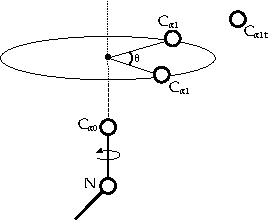
\includegraphics[width=0.85\columnwidth]{figures/ccd_angles}
	\label{fig:ccd_angles}
\end{center}

